\chapter{Contexte général}
    %\addcontentsline{toc}{chapter}{}

\section{Introduction}
Dans ce chapitre, nous présentons l’organisme d’accueil et le cadre dans lequel le projet a été réalisé. Nous décrivons ensuite le contexte général du projet, en soulignant les enjeux liés à la détection des textes générés par l’intelligence artificielle. Enfin, nous expliquons la méthodologie choisie, basée sur l’approche CRISP-DM, pour structurer et guider l’ensemble du projet.
\section{Présentation de l’organisme d’accueil}
Créée en 2010, ESPRIT-Tech est la structure dédiée à la Recherche, Développement et Innovation (RDI) au sein de l’école ESPRIT. Depuis la mise en place des programmes de formation, l’activité RDI est devenue l’une des priorités stratégiques de l’établissement. ESPRIT-Tech regroupe des enseignants-chercheurs et offre un soutien complet en matière de financement, de formation et d’accompagnement dans les projets de recherche. La structure définit les stratégies de recherche en collaboration avec les différentes parties prenantes, en mettant particulièrement l’accent sur l’innovation et la recherche appliquée.
\begin{figure}[h]  % [h] = ici (here)
    \centering
    
\includegraphics[width=0.3\textwidth]{images.png}  % Ajuste la taille avec width
    \caption{Logo d'Esprit-Tech}
    \label{fig:logo}
\end{figure}
\section{Cadre stratégique et valeurs de l’organisme}
ESPRIT-Tech a pour vision de promouvoir la recherche, l’innovation et la valorisation des résultats scientifiques. Elle s’engage à soutenir l’excellence en RDI à travers le développement de projets à fort impact, répondant aux besoins académiques et industriels.
\\
Sa mission consiste à créer un environnement propice à la recherche et à l’innovation, à renforcer le financement externe et à développer un écosystème entrepreneurial ouvert à l’international, favorisant la collaboration entre chercheurs et partenaires.
\\
Les valeurs d’ESPRIT-Tech reposent sur la rigueur scientifique, le respect, l’inclusion et la transparence. Sa démarche s’inscrit dans une logique de coopération, de responsabilité sociale et de développement durable.

\section{Méthodologie CRISP-DM}
CRISP-DM ou Cross-Industry Standard Process for Data Mining, est un modèle de processus qui permet d’orienter les travaux d’exploration de données en data science. 
Cette méthodologie itérative, utilisée par nos data scientist, permet de travailler en cycles : du business understanding pour comprendre le besoin client jusqu’à l’évaluation où l’équipe présente les résultats aux clients et le déploiement. Cette méthode permet de donner un cadre structuré pour guider les data scientist tout au long du cycle de vie d’un projet.
\section{Les étapes de la méthodologie CRISP-DM}
La méthodologie CRISP-DM se compose de 6 étapes clés : 
\\
\\
Etape 1 : La compréhension du besoin client
\\
‍Dans cette phase initiale, l’équipe de data science travaille en collaboration avec les parties prenantes afin de comprendre les objectifs commerciaux, les exigences, les contraintes du projet ainsi que les bénéfices attendus.
Les ressources nécessaires pour réaliser le projet, tels que le budget, les compétences techniques et l'accès aux données, sont évalués. Les problèmes à résoudre sont identifiés et les critères permettant de mesurer le succès du projet sont définis.
Cette étape est essentielle pour garantir la bonne atteinte des objectifs du projet.
\\
\\
‍Etape 2 : La compréhension des données
\\
‍Cette phase consiste à collecter, explorer et évaluer toutes les données disponibles pour le projet. L'équipe de data science analyse ces dernières pour comprendre leur structure, leur qualité, leurs éventuels problèmes, leur pertinence et leur disponibilité. 
Cela permet d’identifier les valeurs manquantes, ou les erreurs qui pourraient affecter les analyses suivantes. Elle se concerte ensuite avec les experts métiers pour identifier des pistes de résolution des problèmes constatés et ainsi aider à interpréter les données.
\\
\\
‍Etape 3 : La préparation des données
\\
‍Une fois que les données ont été évaluées, il faut à présent sélectionner les variables et les échantillons pertinents pour l’analyse, en fonction des objectifs qui ont été fixés.
Les données sont ensuite nettoyées et, si nécessaire, transformées. Cela peut inclure la gestion des valeurs manquantes, l'échantillonnage des données et la création de variables dérivées. Si plusieurs sources de données sont utilisées, elles sont intégrées pour créer un ensemble de données cohérent.
Cette étape monopolise plus de la moitié du temps sur l’ensemble du projet.
\\
‍\\
Etape 4 : La modélisation
‍\\
Dans cette phase, à partir de techniques d'analyse des données, l’équipe de data science construit des modèles prédictifs ou des modèles descriptifs, en fonction des objectifs du projet. Plusieurs itérations ont lieu entre les étapes de préparation et de modélisation pour affiner l’utilisation de certains algorithmes particuliers. 
L’étape du modeling génère souvent plusieurs modèles de Data Mining qui répondent tous à la même problématique.
\\
\\
‍Etape 5 : L’évaluation
‍\\
Une fois que les modèles ont été construits, ils sont évalués pour déterminer leur qualité et leur précision. Cette étape du cycle permet de s’assurer que le modèle permet d’atteindre les objectifs du projet. 
Les performances des modèles sont mesurées à l'aide de métriques appropriées et comparées aux critères de succès définis dans la première phase du cycle. Si les résultats ne répondent pas aux attentes ou s'il y a des problèmes identifiés, les étapes précédentes peuvent être révisées et répétées pour améliorer les performances du modèle
\\
\\
Etape 6 : Le déploiement
‍\\
Enfin, les résultats du projet sont présentés aux parties prenantes et sont intégrés si nécessaire dans les systèmes existants pour aider la prise de décision. Cette phase implique souvent la création de rapports, de visualisations ou d'autres formes de communication pour rendre les résultats compréhensibles et utilisables par ceux qui ne seraient pas spécialistes des données. 
A cette étape, le modèle est performant et répond correctement à la problématique.
\begin{figure}[h]
    \centering
    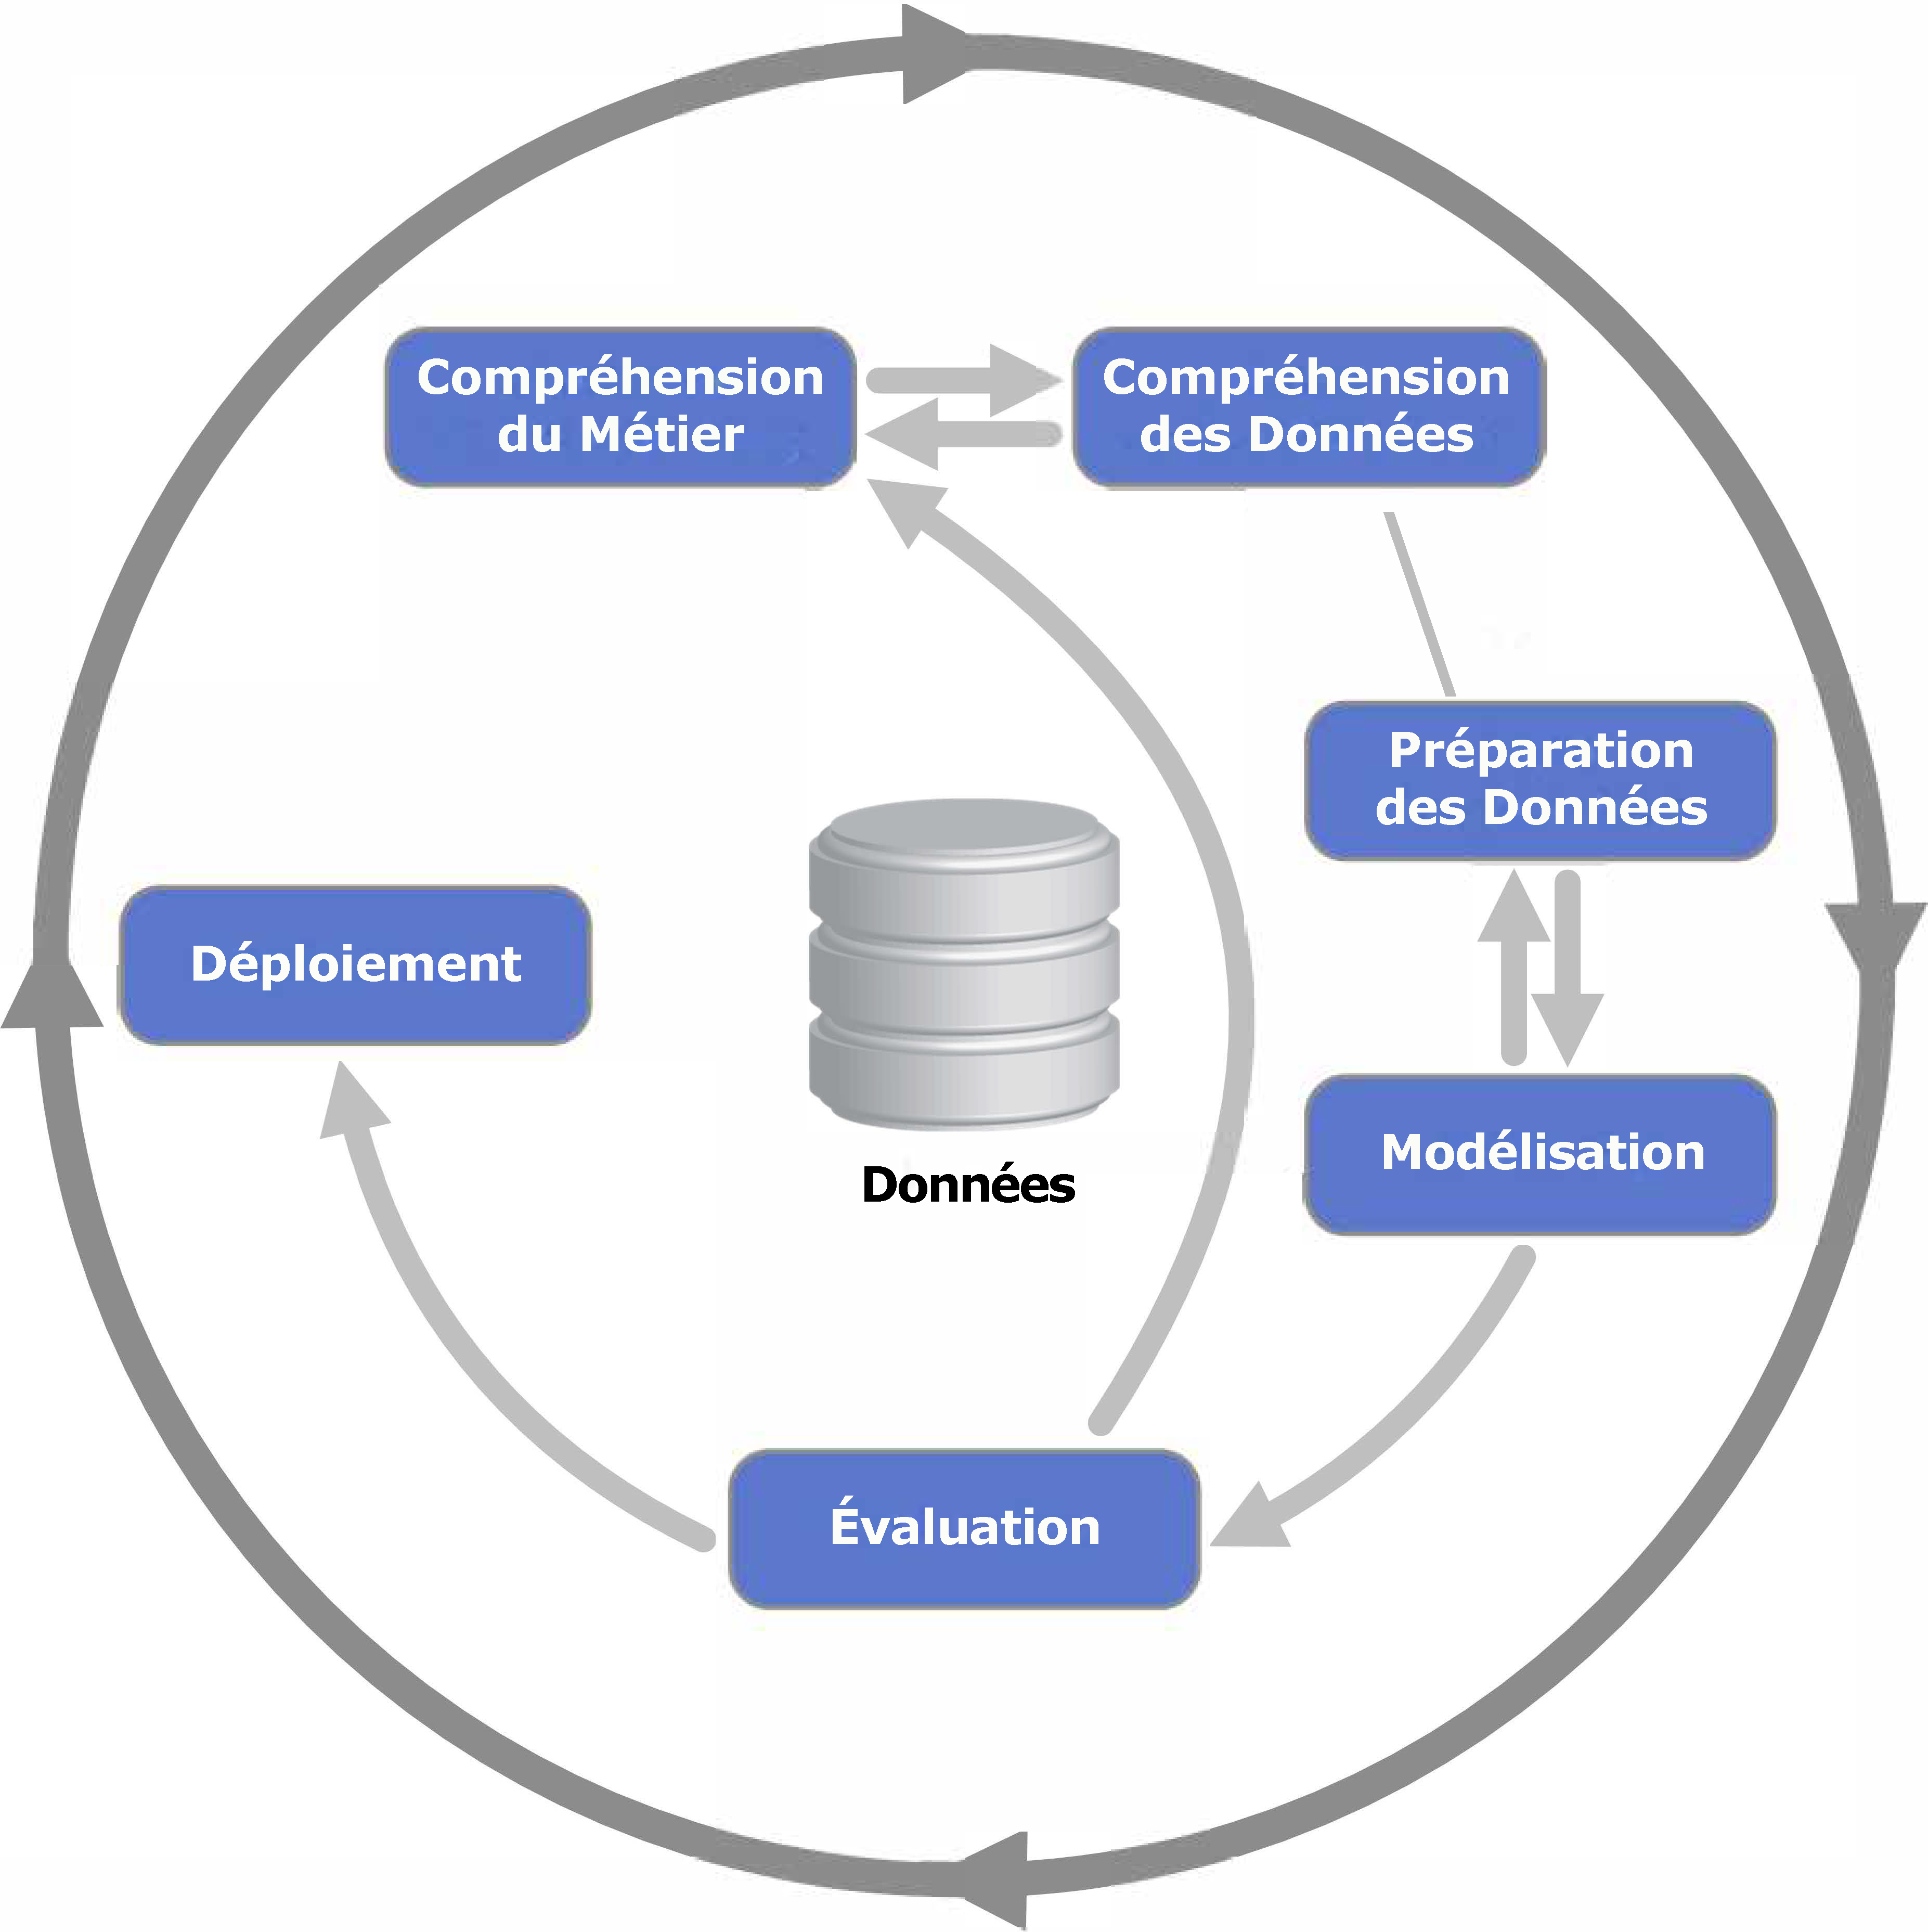
\includegraphics[width=0.5\textwidth]{Diagramme_du_Processus_CRISP-DM.png}
    \caption{Processus CRISP-DM}
    \label{fig:logo}
\end{figure}
\section{Conclusion}
Ce chapitre a présenté ESPRIT-Tech, son rôle, sa vision et ses valeurs, ainsi que le projet de détection de textes IA vs humains, en suivant la méthodologie CRISP-DM pour structurer toutes les étapes du projet. Ces éléments servent de base pour la mise en œuvre et l’évaluation du modèle dans les chapitres suivants.


